\documentclass[a4paper,oneside]{article}
\usepackage{amsmath}
\usepackage{amssymb}
\usepackage{algorithmicx}
\usepackage{graphics}
\usepackage{rotating}

\newtheorem{defi}{Definition}

\title{Measuring Revenue Management Efficiency}
\author{Fedor Nikitin, Antti Tolvanen}

\begin{document}
  \maketitle
  
  \section{Introduction}
  In this paper framework for answering the following questions is provided.
  \begin{enumerate}
    \item How to understand that revenue management done well?
    \item What is efficiency of revenue management?
    \item Is there any reasonable measure of efficiency?
    \item How to follow market movements?
    \item How to separate market performance and revenue management performance on top of the market?
  \end{enumerate}

  \section{Mathematical models}
  \subsection{Static case}
  Let $f_1 > \ldots f_n$ be fares for classes. $f_1$ is the fare of highest class and
  $f_n$ is the fare of lowest class. Demand is characterized by random vector
  $$
  D = (D_1,\ldots,D_n) \sim \mathcal{N}(\mu,\Sigma),
  $$
  where $\mu$ is mean vector and $\Sigma$ is covariance matrix of $n$-dimensional
  multivariate normal distribution on some probability space $(\Omega,\mathcal{F},\lambda)$.

  Let 
  $$
  P = \{ p \in \mathbb{Z}_+^n | \sum_{i=1}^n p_i = c \}
  $$
  be a set of all possible allocations among classes from fixed capacity $c$.
  \begin{defi} Mapping
  $$
  \mathcal{P}_p : \mathbb{R}_+^n \times \mathbb{R}_+^{n\times n} \rightarrow P
  $$
  is called pure strategy.
  \end{defi}
  In other words pure strategy is a function which for each demand vector $\mu$ and covariance matrix $\Sigma$
  assigns certain protection limits.
  \begin{defi} Mapping
  $$
  \mathcal{P}_m : \Omega \times \mathbb{R}_+^n \times \mathbb{R}_+^{n\times n} \rightarrow P
  $$
  is called mixed strategy.
  \end{defi}
  The difference between pure and mixed strategy is that mixed strategy for $\mu$ and $\Sigma$ assigns
  protection limits with some probabilities. Apparently any pure strategy is a mixed strategy.
  \begin{defi}
  Blind strategy is a mixed strategy which is constant in $\mu$ and $\Sigma$ and independent of $D$.
  \end{defi}

  Revenue under some mixed strategy $\mathcal{P}_m(\omega) = (p_1(\omega),\ldots,p_n(\omega))$ is given by
  $$
  R(\mathcal{P}_m) = \sum_{i=1}^n f_i \cdot \min\{ D_i(\omega), p_i(\omega) \}
  $$
  and is, indeed, random variable with some distribution.

  Consider also
  $$
  \hat{R}(\mathcal{P}_m) = \sum_{i=1}^n f_i \cdot \min\{ \mu_i, p_i(\omega) \}.
  $$

  When demand gets detereministic, i.e. $\Sigma$ is identity matrix then
  $$
  R(\mathcal{P}_m) = \hat{R}(\mathcal{P}_m).
  $$

  \begin{defi}
  Blind performance is
  $$
  BP = E[R(\mathcal{P}_b)]
  $$ 
  \end{defi}

  \begin{defi}
  Blind volatility is
  $$
  BV = \sqrt{Var(R(\mathcal{P}_b)}
  $$
  \end{defi}

  \begin{defi}
  Market volatility is
  $$
  MV = BV - \sqrt{Var(\hat{R}(\mathcal{P}_b))}
  $$
  \end{defi}

  Suppose actual realized revenue is
  $$
  R = \sum_{i=1}^n f_i \cdot b_i.
  $$
  
  \begin{defi}
  Efficiency is
  $$
  \epsilon = \frac{R - BP}{BV}.
  $$ 
  \end{defi}

    \subsection{Dynamic case}

  \section{Applications}
    \subsection{Revenue Mangement Efficiency}
    \subsection{Test for skills}
    \subsection{Risk awarness and VaR}  

  \section{Implementation}
  To calculate $\epsilon$ we need to find distribution of random variable
  $R(\mathcal{P}_b)$. Potentially given certain blind strategy one can
  find closed-form of probabily density function of $R(\mathcal{P}_b)$.

  In general much easier approach is to simulate random variable
  $R(\mathcal{P}_b)$ and consider sample mean and sample variance as 
  estimates for $BP$ and $BV$. 

  If $n$ is the number of booking classes and $m$ is the number of simulation runs
  then complexity of algorithm is $O(nm)$.

  \section{Discussion}

  Approach is taken above to define revenue management efficiency is borrowed
  from portfolio theory. Random portfolios are used there to analyze and give score
  to investment funds or particular portfolio managers. Idea is simple knowing past
  history of the market one could ask what if porftolio was managed in completely 
  random fashion and not utilizing any knowledge of the market. Random fashion means
  here that at each point of time decisions to sell or to buy were done independently
  of market signals. Simulating this random behavior using past history yields the 
  value of the portfolio on current date. This simulated value is compared then with
  actual realized value of portfolio and the gap between these two values gives an idea
  of performance of certain mutual fund or manager.

  One of advantages of this method is that it allows to separate market changes and
  performance of manager. Value of random portfolio incorporates information on 
  the market change and serves as reliable benchmark to measure the performance.
  Traditional benchmarks as compare-to-last-year are lacking this property.

  Application of idea from portfolio theory to revenue management is straightforward.
  Suppose when flight departed we are given forecast of demand for each class and
  actual bookings in each class. Question we want to answer is whether the flight was 
  managed well. In the same way as in portfolio theory we define random fashion of 
  managing the flights which is the process of assigning protection limits not 
  utilizing any knowledge of forecast. Simulating this random behavior of revenue
  manager brings some average revenue which is achieved in current market conditions
  when no revenue management is applied. The difference between actual revenue and 
  simulated revenue estimates revenue added by revenue management practice. In order
  to compare this measure across different markets and time we scale it by variance 
  of simulated revenue.   

  Some notes on formal definitions. Demand is assumed to follow joint normal distribution,
  but components could be dependent. This is done to stress that the proposed approach 
  handles both cases dependency and indepedency easily. Assumption of normalilty is not
  restriction either. We made this assumption basically for the ease of introduction further 
  definitions. 

  Joint normal distribution is fully defined by mean vector and covariance matrix. That is why
  we define pure strategy as mapping from the set of all possible mean vectors and covariance
  matrices to the set of all possible class protections. Notice that nesting order of classes
  is ignored and protection for the class is just the number of bookings we aim to get to this 
  class. We believe that using nesting protection limits will just complicate formulas, but
  will not lead to different theoretical results.

  We define mixed strategy in order to model random behavior in defining protection limits.
  To our knowledge mixed strategies are not discussed in revenue management literature, but
  they are well studied and used in general optimization theory. They idea behind them is
  quite simple. Given some knowledge of the market one could artificially randomize his/her
  behavior. Under certain conditions mixed strategy could do better, but not in classical
  revenue management settings. Difference of definition compared to pure strategies is just
  dependency of protection limits on realization of random event ($\omega \in \Omega$).  

  Blind strategy is model for random behavior not utilizing any knowledge of the market.
  We define it constant in mean vector and covariance matrix and independent of demand.
  Fact that it is not utilizing any knowledge of the market is justified by the fact
  it is the same for different market conditions (mean vector and covariance matrix).
  Independence of demand and strategy is natural due to realization of demand vector
  should not anyhow affect the way strategy chosen.

  Blind performance is defined naturally through average result achieved with blind
  strategy. We associate blind performance with market performance. We believe that
  it is market characteristic and revenue management actions are eliminated through
  randomization. When it grows it tells about growing market and other way around
  when it falls it tells us about falling market.
  Blind volatility characterize variability of random blind result. This
  incorporates both variability of the market as well as variability of the result
  due to random management procedure.

  Efficiency measure tells how many times measured in the number of standart deviations
  achieved result is better than result achieved with blind random behavior.
  We separate blind volatility and market volatility. The reason for this is that
  blind volatility contains also volatility due to blind strategy. To separate
  market volatility and blind volatility we define revenue achieved with mixed strategy and 
  deterministic demand (see $\hat{\mathcal{R}}$). We take the difference (?) and call
  it market volatility.

  Advantages:
  \begin{itemize}
    \item Always defined (low and high demand flights).
    \item Easy to calculate.
    \item Accounts for statistical properties of demand.
    \item Could be implemented for any type of demand (normality
    is not restriction).
  \end{itemize}
  Disadvantages:
  \begin{itemize}
    \item Assumes good forecast.
    \item Understanding of the measure requires familarity with concept of probability.
  \end{itemize}
  \section{Experiments}
  We made simulation of one Finnair flight to BKK for the last year. Picture with
  graphs is below. On the first graph there is two time series. Green one is actual
  revenue (PIF multiplied by the number of bookings on departure date) and simulated
  blind revenue. It is seen that actual revenue is always above of simulated revenue,
  but there is some periods when the distance between actual and simulated one is quite
  small. This indicates that in these periods revenue management could be improved.
  Good example of this time period is period just before Christmas last year. Simulated
  revenue is very close to actual one. On other hand there are also positive examples
  when for falling down market revenue management was adjusted such that efficiency
  stayed on the same level. 

  Second graph plots defined above efficiency measure and the last one plots 
  market volatility defined above as well.

  \begin{sidewaysfigure} 
   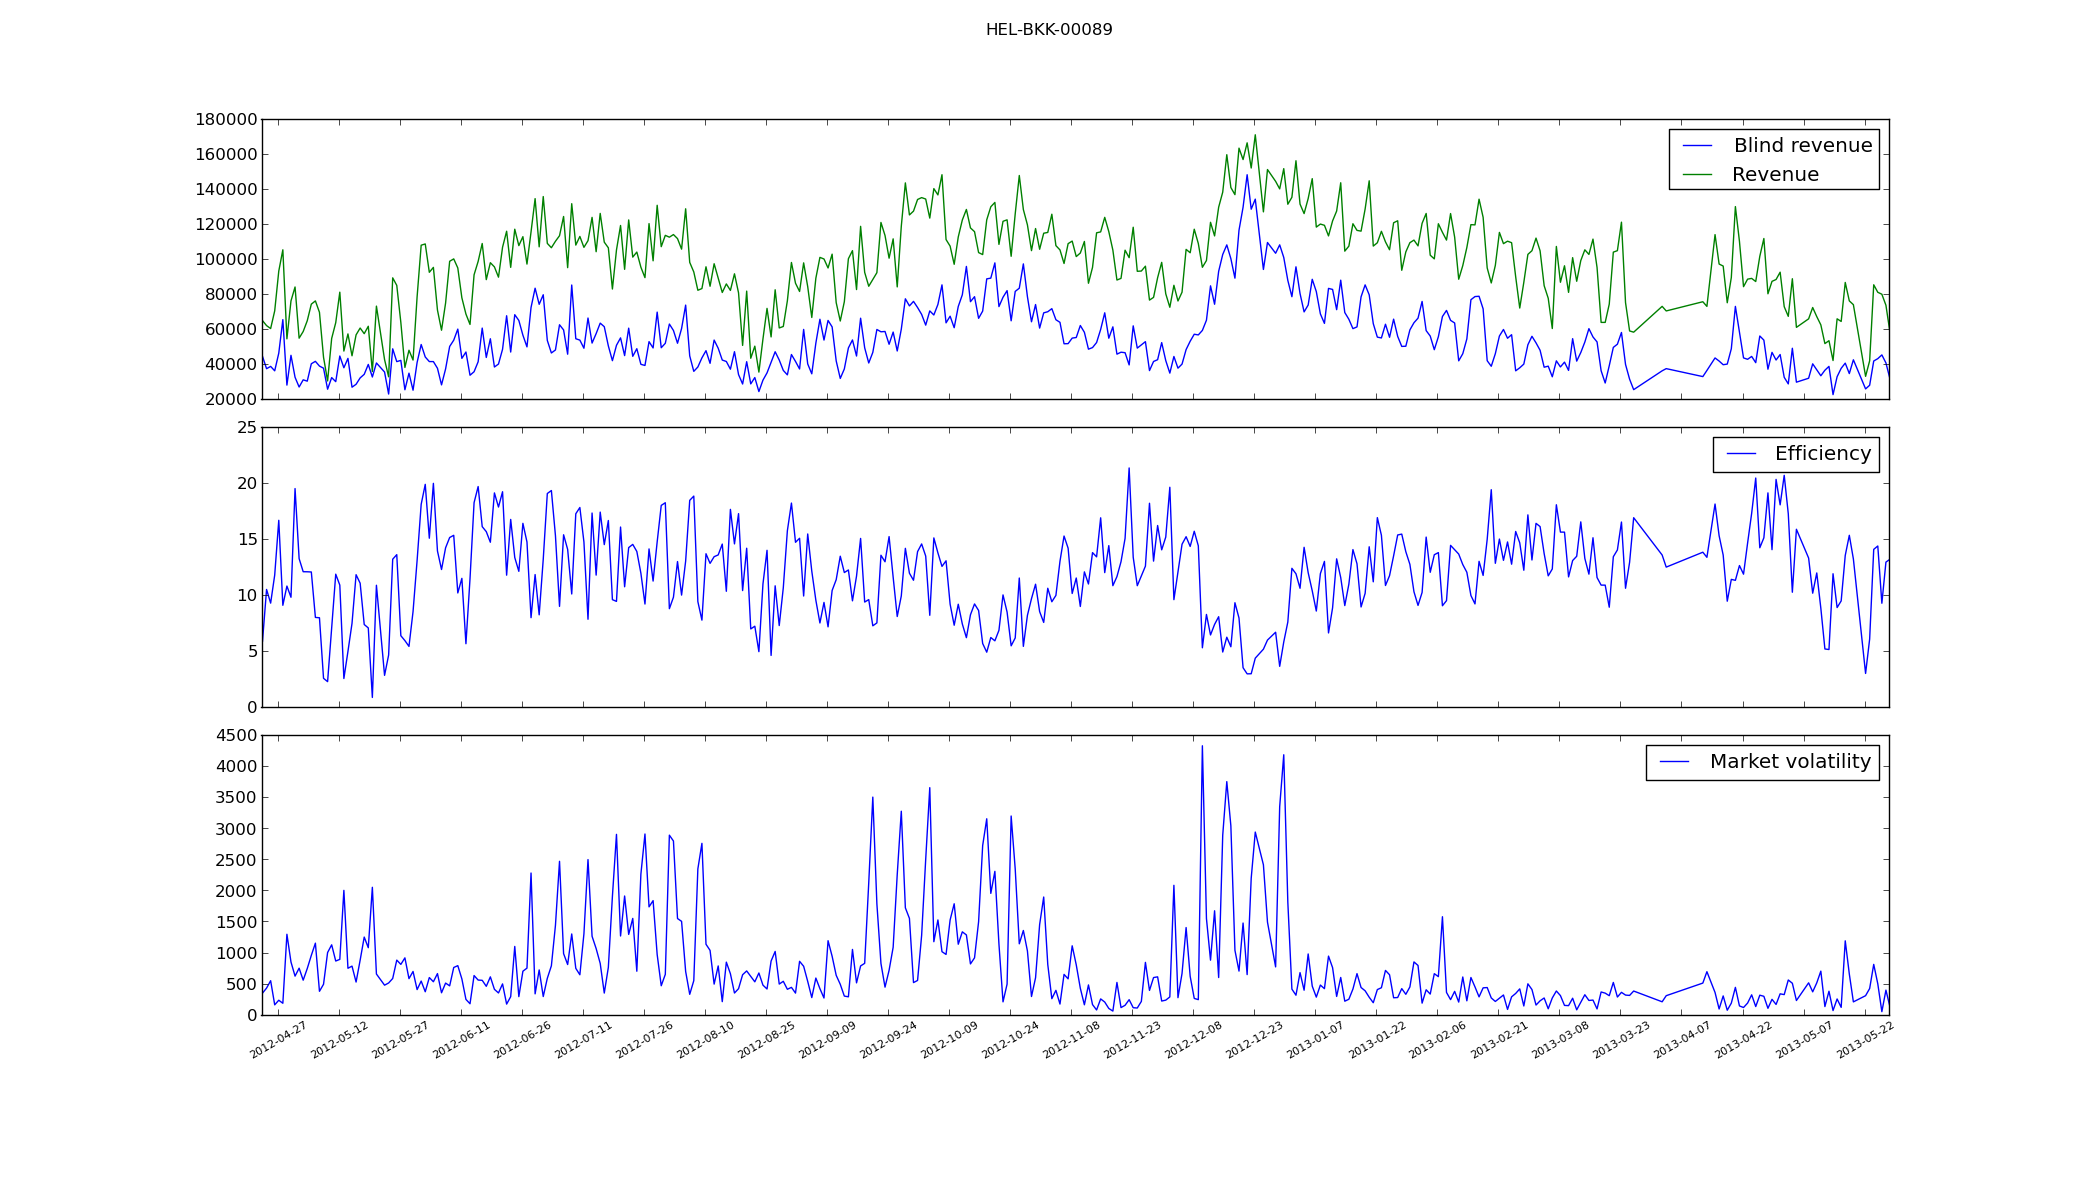
\includegraphics[width=700px,height=400px]{89.png}
  \end{sidewaysfigure} 

  \begin{thebibliography}{9}

    \bibitem{sumkin13} Sumkin is kot.

  \end{thebibliography}
  
\end{document}
